%\documentclass[tikz,convert={outfile=\s1.svg}]{standalone}
\documentclass[tikz]{standalone}
\usepackage{amsthm}
\usepackage[landscape]{geometry}
\usepackage{multicol}
\usepackage{tikz}
\usepackage{pgfplots}
\usepackage{xcolor}
\usepackage{amsmath}
\usepackage[T1]{fontenc}
\usepackage{utopia}
\usepackage{changepage}
\usepackage{amssymb}
\usepackage{fancyhdr}
\usepackage[many]{tcolorbox}
\usepackage{moresize}
\usepackage{fullpage}
\usepackage{mathpazo}
\usepackage{tikz-3dplot}
\usepackage{cancel}
\tdplotsetmaincoords{70}{165}
\pgfplotsset{compat=1.18}
\usepackage{enumitem}
\usepackage{tabularray}
\usepackage{mathtools}

\UseTblrLibrary{diagbox}

\usetikzlibrary{
    shadings, calc, patterns, angles, quotes, arrows.meta, 
    decorations.pathmorphing, decorations.pathreplacing, 
    fadings, 3d, perspective, backgrounds, intersections, 
    decorations.markings, bending, positioning, 							spy,shapes.geometric,shadows,shapes.symbols, fadings, matrix, fit
}

\usepgfplotslibrary{
    groupplots, external, colormaps, patchplots, fillbetween
}


% Reds (r)
\definecolor{r1}{RGB}{255, 191, 191}    % Light coral
\definecolor{r2}{RGB}{255, 191, 223}    % Light pink
\definecolor{r3}{RGB}{255, 207, 207}    % Light rose

% Blues (b)
\definecolor{b1}{RGB}{191, 223, 255}    % Light blue
\definecolor{b2}{RGB}{191, 239, 255}    % Light sky
\definecolor{b3}{RGB}{191, 255, 255}    % Light cyan

% Greens (g)
\definecolor{g1}{RGB}{191, 255, 191}    % Light green
\definecolor{g2}{RGB}{191, 255, 223}    % Light mint
\definecolor{g3}{RGB}{207, 255, 207}    % Light sage

% Oranges (o)
\definecolor{o1}{RGB}{255, 223, 191}    % Light peach
\definecolor{o2}{RGB}{255, 239, 191}    % Light cream
\definecolor{o3}{RGB}{255, 231, 191}    % Light buff

% Violets (v)
\definecolor{v1}{RGB}{223, 191, 255}    % Light purple
\definecolor{v2}{RGB}{239, 191, 255}    % Light lilac
\definecolor{v3}{RGB}{231, 191, 255}    % Light lavender

% Yellows (y)
\definecolor{y1}{RGB}{255, 255, 191}    % Light yellow
\definecolor{y2}{RGB}{255, 247, 191}    % Light cream yellow
\definecolor{y3}{RGB}{255, 239, 191}    % Light warm cream

\definecolor{w}{HTML}{eeeeee}
\definecolor{g}{HTML}{444444}
\definecolor{b}{HTML}{222222}
\definecolor{lightgrey}{HTML}{cccccc}
\definecolor{firebrick}{RGB}{178, 34, 34}
\definecolor{myg}{RGB}{3, 252, 177}


\color{w}
\begin{document}
\ssmall
%\pagecolor{b}
\nopagecolor
\fontfamily{put}

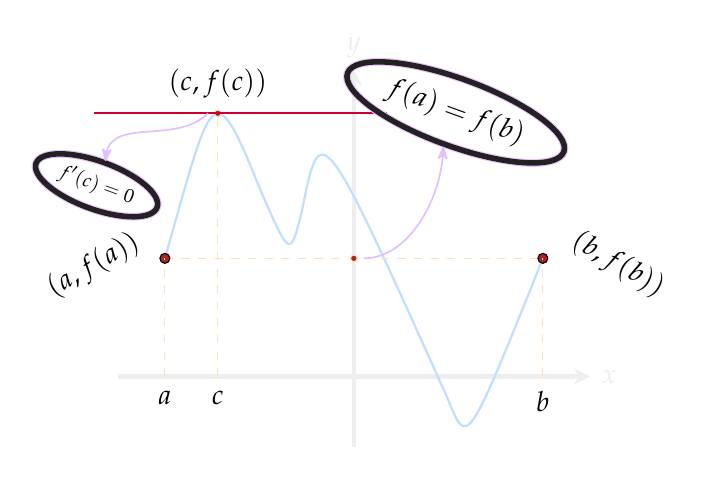
\begin{tikzpicture}[scale=0.6]
	\draw[ultra thick, -stealth, w] (-4-1, 0) -- (-4+9, 0) node[right] {$x$};
	\draw[ultra thick, -stealth, w] (0, 2.5-4) -- (0, 2.5+4) node[above] {$y$};
	\draw[thick, draw=b1] 
	(-4, 2.5) .. controls +(1, 3.5) and +(-1, 2.5) .. +(2, 1.5)
	.. controls +(0.65, -1.5) .. +(2.9, 1) 
	.. controls +(0.4, 2) .. +(6, -3)
	.. controls +(0.4, -1) .. +(8, 0);
	
	\draw[dashed, draw=o1] (-4, 2.5) -- +(8, 0);	
	
	\filldraw[fill=firebrick] (-4, 2.5) circle(3pt);
	\node[outer sep=2pt, above left, rotate=30] at (-4, 2.5) {$(a, f(a))$};
	\node[outer sep=2pt, below] at (-4, 0) {$a$};
	\draw[draw=o1, dashed] (-4, 0) -- (-4, 2.5);
	
	\filldraw[fill=firebrick] ($(-4, 2.5) + (8, 0)$) circle(3pt);
	\node[outer sep=3pt, above right, rotate=-30] at ($(-4, 2.5) + (8, 0)$) {$(b, f(b))$};
	\node[outer sep=2pt, below] at ($(-4, 0) + (8, 0)$) {$b$};
	\draw[draw=o1, dashed] ($(-4, 0) + (8, 0)$) -- ($(-4, 2.5) + (8, 0)$);
	
	\filldraw[draw=o1, fill=firebrick] ($(-4, 2.5) + (1.12, 3.07)$) circle (2pt);
	\draw[draw=blue!20!red, thick] (-4 - 1.5, 2.5 + 3.07) -- (-4 + 4.7, 2.5 + 3.07);
	\node[outer sep=2pt, above] at ($(-4, 2.5) + (1.12, 3.07)$) {$(c, f(c))$};
	\node[outer sep=2pt, below] at (-4 + 1.12, 0) {$c$};
	\draw[draw=o1, dashed] (-4 + 1.12, 0) -- (-4 + 1.12, 2.5 + 3.07);
	
	\node[] (val) at (0, 2.5) {};
	\filldraw[draw=o1, fill=firebrick] (0, 2.5) circle (2pt);
	\node[draw=v2, below left, outer sep=1pt, rotate=-20, shape=ellipse, double=b, double distance=2pt] (vals) at ($(0, 2.5) + (4, 3)$)  {$f(a) = f(b)$};
	\draw[->, draw=v1, >={Stealth[round]},semithick] (val.east) .. controls +(right:1cm) and +(down:1cm) .. (vals.south);
	
	\node[] (cp) at ($(-4, 2.5) + (1.12, 3.07)$) {};
	\node[scale=0.7, draw=v2, below left, outer sep=1pt, rotate=-20, shape=ellipse, double=b, double distance=2pt] (cps) at ($(-4, 2.5) + (1.12, 3.07) + (-1.5, -1.5)$)  {$f'(c) = 0$};
	\draw[->, draw=v1, >={Stealth[round]},semithick] (cp.west) .. controls +(225:1cm) and +(up:1cm) .. (cps.north);
\end{tikzpicture}
\end{document}ls